\newpage{\thispagestyle{empty}\cleardoublepage}
\chapter{dyngen: simulating single cells} 
\chaptermark{dyngen: simulating single cells}
\label{chap:dyngen}

\begin{quote}
	\textbf{Abstract:} 
\end{quote}

\vfill

Adapted from:\\

\newpage

\section{Introduction}
Continuous technological advancements to high-throughput profiling of single cells
are having profound effects on how researchers can validate biological hypotheses. 
For example, single-cell RNA sequencing (scRNA-seq) directly resulted in the development
of a new type of computational method called trajectory inference (TI). By profiling
the transcriptomics profiles of developing cells, TI methods attempt to reconstruct 
and characterise the underlying dynamic processes \cite{cannoodt_computationalmethodstrajectory_2016}.
While early experimental technologies allowed to profile one single modality (e.g. DNA sequence, 
RNA or protein expression), recent developments permit profiling multiple modalities simultaneously.

An ideal experiment would be able to observe all aspects of a cell, including a full history of its 
molecular states, spatial positions and environmental interactions \cite{stuart_integrativesinglecellanalysis_2019}. 
While this falls outside the reach of current experimental technologies, \textit{in silico} simulations
of single cells would allow developing the next wave of computational techniques
in anticipation of new experimental technologies.

A few generators of scRNA-seq profiles have already been developed (e.g. splatter \cite{zappia_splattersimulationsinglecell_2017} and PROSSTT \cite{papadopoulos_prossttprobabilisticsimulation_2018}). These can be 
used to evaluate the performance of computational tools, and to explore their strengths and weaknesses. A limitation of directly simulating a scRNA-seq profile (instead of a single cell) is that extending the simulation to other aspects of the cell -- such as tracking the full history of molecular states -- becomes difficult.


\section{Results}

dyngen is a simulator for single cells that develop over time. Each cell contains an underlying gene regulatory network (GRN) that specifies which chemical reactions can occur at any given point in time, depending on the availability of required molecules (Figure \ref{fig:dyngen}A).
It was initially developed as part of a comprehensive benchmark of TI methods \cite{saelens_comparisonsinglecelltrajectory_2019} but has since been extended to be applicable in a much broader context. 
One main improvement is being able to profile multiple aspects of a single cell at any given time point: its molecule abundance levels, which reactions took place, and which parts of the gene regulatory network were active. The underlying GRN allows dyngen to be used in a variety of experimental scenarios in order to evaluate many different types of computational tools (Figure \ref{fig:dyngen}B).

\begin{figure}
	\centering
	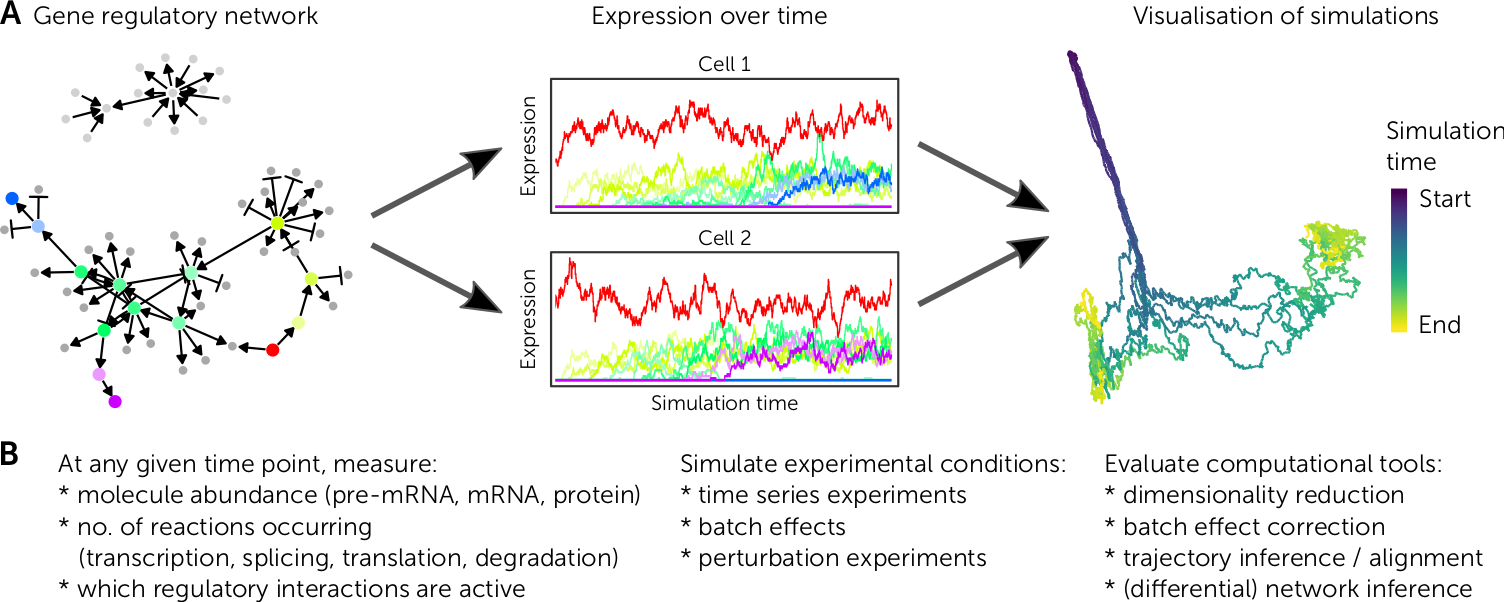
\includegraphics[width=\LARGEfigure]{fig/dyngen/showcase_3.png} 
	\caption{Showcase of dyngen functionality. \textbf{TODO: change to pdf.}} % TODO: update label
	\label{fig:dyngen}
\end{figure}

\subsection{Example simulation}

\subsection{Applications}

\subsection{Supported backbones}

\subsection{Backbone lego}

\subsection{Additional experimental effects}
% time series, batch effects, perturbation experiments


\section{Discussion}

\section{Methods}










%dyntoy and PROSSTT are specifically developed to generate datasets
% containing single cells which develop along a certain trajectory.
% These generators start a certain topology in mind, 
% simulate changing gene expressions along each of the branches of the topology, and sample cells
% from random points in the trajectory. splatter is focused on well replicating the specific noise characteristics of
% scRNA-seq data, and simulates differentially expressed genes in order to replicate clusters of cells, batch effects
% and even trajectories. dyngen 1.0 borrows a page from GeneNetWeaver in that it also converts a GRN into an ODE, but
% the GRN is constructed in such a way that the repeated simulations resemble single cells following a regulatory program
% (e.g. differentiation into one of two celltypes). BoolODE uses the dyngen 1.0 GRNs but uses boolean models to convert 
% the network into an ODE, and is used to evaluate the performance of NI methods, not TI methods. 

%\begin{table}
%	\caption{\textbf{Comparison of existing single-cell omics simulators.} TI: trajectory inference, NI: network inference, Cl: clustering, DR: dimensionality reduction.} \label{tab:simulators}
%	\centering\fontsize{9}{11}\selectfont
%	\begin{tabularx}{\linewidth}{p{1.6cm}p{2.5cm}p{3cm}X}
%		Generator & Used to evaluate & Data type(s) & Approach \\ \hline
%		dyngen 1.0 & TI & mRNA \& protein & GRN, ODE, Euler--Maramuya \\
%		dyntoy & TI & mRNA & Visualise tree in plane, generate expression in plane, sample cells from tree \\
%		PROSSTT & TI & mRNA & Random walks along tree, sample cells from tree \\
%		splatter & Cl \& TI & mRNA & Simulate DE genes, simulate scRNA-seq noise \\
%		BoolODE & NI & mRNA \& protein & Use dyngen GRN's, ODE, Euler--Maramuya \\
%		dyngen 2.0 & TI, NI, Cl, DR & pre-mRNA, mRNA, protein & Backbone, GRN, SSA \\
%		dyngen 3? & TI, NI, Cl, DR & pre-mRNA, mRNA, miRNA, protein, protein complex & Backbone, GRN, SSA
%	\end{tabularx}
%\end{table}